\section{Simple Configurable Classifiers}
\label{sec:conjecture}

We argue that continuous mobile sensing applications should be
structured as a pair of classifiers of increasing complexity: a simple
high recall and moderate precision classifier that runs continuously
on low-power hardware, and acts as an energy efficient wake-up
mechanism for a higher complexity classifier that runs on the main CPU
and provides both high recall and high precision.

We conjecture: 1) that it is possible to implement simple classifiers for a 
wide range of applications by configuring a small set of common processing 
algorithms; and  2) that this approach will achieve comparable energy 
savings to an alternative implementation that supports full programmability.

\subsection {Approach}

{\em Simple Configurable Classifiers} (SCC) is a new approach for
continuous mobile sensing that divides the responsibility of
energy-efficient event detection between the platform and
the application developer.  The platform implements common sensor data
processing algorithms that execute on a low-power sensor hub.
Applications construct simple classifiers for events of interest by
selecting among the set of pre-defined 
algorithms and tuning their parameters.  This classifier executes on
the low-power sensor hub and, when events of interest are detected,
the main processor is woken up and the application code is invoked.
  
Figure~\ref{fig:architecture} shows the architecture of a
system that features SCC. Applications interact with a sensor 
manager to define simple configurable classifiers. A simple 
classifier is assembled out of a series of data processing
algorithms, where the output of one algorithms becomes the input to
the next one, similar to a pipeline.  Common algorithms
that perform data windowing, cleaning, filtering, feature extraction 
or admission control would be used as building blocks for the 
pipeline.  The figure also
shows that the architecture supports recognition libraries that
encapsulate the functionality of SCC to provide simple
wake-up conditions and event detection for a large number of activities. 

While determining the set of algorithms to include as part 
of the platform is an open research questions that is beyond the scope 
of this paper, we anticipate that this set will include popular 
algorithms such as moving averages, low and high-pass filters, and Fast 
Fourier transform, among others.


\begin{figure}[t]
	\centering
	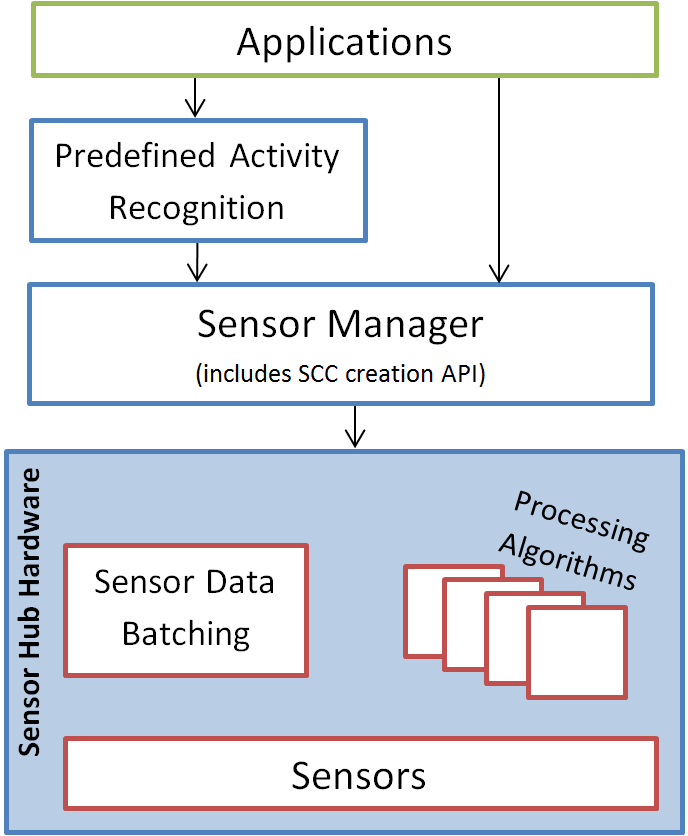
\includegraphics[width=3.1in]{architecture.png}
	\caption{Proposed system architecture.}
    \label{fig:architecture}
\end{figure}

\subsection{Advantages}

SCC has many benefits:

 {\bf Lower programming complexity}  Programming complexity is
  decreased because application developers can use the pre-defined
  processing algorithms, rather than implementing them themselves. 
  Application developers need to select appropriate processing 
  algorithms for their pipelines and configure their parameters. This 
  is not unlike how shell programming is used to build complex 
  pipelines by reusing existing command-line applications.
  

{\bf Better predictability} It 
  creates predictable performance for the algorithms executed on the
  low-power processor. Profiling each algorithm will provide metrics
  about computational and time requirements, as well as power
  consumption.  Predictable performance is important in order to
  support multiple concurrent classifier executions or applications
  that make use of multiple sensors.


{\bf Better security} Providing access to these algorithms via
  an API has significant security advantages over the fully
  programmable offloading approach because application developers
  cannot execute arbitrary code on the peripheral processor. 


{\bf Improved Portability} Programmers do not have to be
  aware of the specifics of the underlying hardware, nor create a version
  for every type of sensor hub. Since the algorithms are
  pre-specified, device manufacturers can optimize their
  implementations for each low-power processor and sensor
  implementation.



\subsection{Challenges}
\label{sec:challenges}

There are many challenges that will have to be resolved in order to
make SCC possible:

{\bf Identifying processing algorithms} Defining the appropriate
set of algorithms that should be included in the API and executed on
the low-power processor for each sensor is a key challenge. First,
there is a trade-off between algorithm generality and accuracy.
Simple generic algorithms can support a large set of
applications, albeit no specific application is likely to experience
optimal performance.  Conversely, a highly specialized algorithm may
provide optimal performance but is only applicable to a limited set of
applications.  Second, there is also a trade-off between algorithm
complexity and power savings.  More complex algorithms can reduce
energy consumption by preventing unnecessary wake-ups due to increased
accuracy. On the other hand, more complex algorithms have higher
computational demands, which require a larger and hungrier peripheral
processor.

{\bf Access to sensor data} A related challenge is determining what
data the sensor hub should pass to the application following a
wake-up. Some applications may be interested in the raw sensor data,
while others may want to use the filtered data or extracted features.
An across-the-board solution would be to allow the applications to
specify what data they are interested in via the API.

{\bf Configuring classifiers} We believe application developers may
face challenges in selecting the optimal algorithms and configuration
parameters for their simple classifiers.  Given feedback from the
application, self-learning mechanisms may be able to determine optimal
configuration parameters for the algorithms used.  It is easy to 
imagine an application notifying the
sensor hub about wake-ups when events of interest were not actually
detected (i.e. false positives).  However, it will be more difficult
to automatically identify events of interest missed by the classifier
running on the low-power node (i.e. false negatives).

{\bf Multi-application support} Another challenge lies in supporting
multiple concurrent applications while still maintaining predictable
performance.  This challenge is not unique to our approach; however,
given that the algorithms in our approach are pre-defined, they can be
profiled in terms of computational power requirements.  A resource
manager would be required to orchestrate and synchronize concurrent
requests from multiple applications.

{\bf Sizing} Determining the optimal number, type and size of
processors to include in the sensor hub is an open research question.
Each sensor (or small group of related sensors) may be supported by
its own dedicated low-power processor.  Alternatively, a larger
processor could be used to serve the entire sensor hub.  Identifying a
sweet spot between the maximum number of concurrent algorithm
executions, energy budget, cost and physical size of the sensor node
is an open challenge.

{\bf Sensor fusion} Fusing inputs from multiple sensors is a common
technique used for improving the accuracy of sensing applications.
Whether low power sensor hubs should include support for sensor
fusion, however, is not clear.  On the one hand, such support could
increase energy efficiency by reducing the occurrence of unnecessary
wake-ups.  On the other, sensor fusion tends to be application specific
and the added complexity may negate any energy benefits.

